\titre{Exemple : ARP spoofing} \\

\titre{Définition :} Man in the Middle est un terme générique désignant une attaque où l'attaquant peut accéder en lecture et en écriture à toutes les données circulant entre deux machines. \\

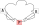
\includegraphics[width=100px]{Images/05_MIM.pdf}\\
A et B pensent qu'ils communiquent directement alors que toutes les données passent par P.\\

\titre{ARP spoofing} A et B sont reliés par l'intermédiaire d'un commutateur.

\titre{Rappel : fonctionnement d'un commutateur}\\
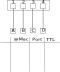
\includegraphics[width=100px]{Images/06_commutateur.pdf}\\
Lorsqu'on aliment le commutateur la table est vide. 
\par Le commutateur remplit sa table en inspectant les adresses MAC sources des trames qui circulent.
\par Si l'adresse MAC source n'est pas présente dans la table, il renvoie la trame sur tous les ports.

\titre{Exemple :}\\
\includegraphics[width=300px]{Images/07_exemple.pdf}\\
\begin{itemize}
	\item A envoie à B
	\item E envoie à F
	\item B envoie à E
	\item G envoie à E
\end{itemize}

\begin{itemize}
	\item Table de SW0
	\begin{tabular}{|l|l|l|l|} \hline
		MAC & Port & TTL & Méthode\\ \hline
		@A & 1 & 100 & Flooding \\ \hline
		@E & 5 & 100 & Flooding \\ \hline
		@B & 2 & 100 & Forwarding port 5\\ \hline
	\end{tabular}

	\item Table de SW1
	\begin{tabular}{|l|l|l|l|} \hline
		MAC & Port & TTL & Méthode\\ \hline
		@A & 1 & 100 & Flooding \\ \hline
		@E & 2 & 100 & Flooding \\ \hline
		@B & 1 & 100 & Forwarding port 2 \\ \hline
		@G & 4 & 100 & Forwarding port 2 \\ \hline
	\end{tabular}
\end{itemize}

\titre{Rappel : fonctionnement du protocole ARP et du modèle OSI} 
	\begin{itemize}
		\item Couches : 
			\begin{itemize}
				\item Application
				\item Transport - Fiabilité de bout en bout - TCP
				\item Réseau - Trouver le chemin - IP
				\item Liaison - Dépend du média et permet d'assurer une transmission fiable sur ce média - Ethernet, Wifi etc.
				\item Physique - Caractéristiques mécaniques et électriques du média et es signaux circulant dessus
			\end{itemize}
		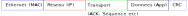
\includegraphics[width=300px]{Images/09_OSI.pdf}
		\item ARP(Adress Resolution Protocol) permet de connaitre l'adresse MAC d'une machine, connaissant son adresse IP. Le fonctionnement générique : envoi d'une requête ARP en broadcast, la machine qui reconnait son IP répond.\\
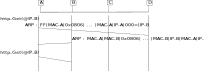
\includegraphics[width=300px]{Images/10_ARP.pdf}\\

	\end{itemize}

\titre{ARP spoofing :} spoofing ou cache poisonnig = usurpation

\titre{Méthode 1 :} Le pirate envoie des réponses ARP en continu.
\begin{itemize}
 \item Réponse émise à destination de A : \\
	@MAC-A|@MAC-P|0x0806| \ldots | @MAC-P | @IP-B | @MAC-A | @IP-A | \ldots
 \item Exemple de trame envoyée par A à destination de B \\
	@MAC-C|@MAC-A|0x0800| ....|@IP-A|@IP-B| .... 
 \item Réponse émise à destination de B : \\
	@MAC-B|@MAC-P|0x0806| \ldots | @MAC-P | @IP-A | @MAC-B | @IP-B | \ldots
 \item Exemple de trame envoyée par B à destination de A \\
	@MAC-C|@MAC-B|0x0800| ....|@IP-B|@IP-A| .... 
\end{itemize}

\titre{Méthode 2 :} Le pirate envoie des requêtes ARP en continu. En effet, dès qu'une machine reçoit une requête, elle enregistre les infos sur la source dans son cache ARP. \\
	Trames émises par C 
	\begin{itemize}
		\item @MAC-A | @MAC-C | 0x0806 | \ldots | @MAC-C | @IP-B | 00 | IP-A
		\item @MAC-B | @MAC-C | 0x0806 | \ldots | @MAC-C | @IP-A | 00 | IP-B
	\end{itemize}

\titre{Comment l'éviter ?} Segmenter le réseau (ne pas rester tous sur le même média). On isole les différents groupes d'utilisateurs (60 machines maximum sur un même segment).

